\documentclass[conference]{IEEEtran}

\usepackage{cite}
\usepackage{amsmath,amssymb,amsfonts}
\usepackage{graphicx}
\usepackage{booktabs}
\usepackage{array}
\usepackage{textcomp}
\usepackage{xcolor}
\usepackage[hidelinks]{hyperref}

\usepackage{bm}
\newcommand{\qhat}{\hat{q}_{\alpha}}

\begin{document}

\title{Adaptive Interval Calibration for DeepPIPE under\\
Distribution Shift: Two-Phase Training and State-Dependent\\
Conformal Control on the NIFTY~50}

\author{%
\IEEEauthorblockN{Raunak Goyal}
\IEEEauthorblockA{Dept.\ of Computer Science and Engineering\\
\texttt{raunak.goyal@example.edu}}
\and
\IEEEauthorblockN{Anshul Saxena}
\IEEEauthorblockA{Dept.\ of Computer Science and Engineering\\
\texttt{anshul.saxena@example.edu}}
\and
\IEEEauthorblockN{Snehanshu Baneerjee}
\IEEEauthorblockA{Dept.\ of Computer Science and Engineering\\
\texttt{snehanshu.baneerjee@example.edu}}
}

\maketitle

\begin{abstract}
Distribution-free prediction intervals are attractive for financial forecasting because they do
not assume a parametric error model, yet their reliability under distribution shift remains
poorly understood. We study \emph{DeepPIPE}---an encoder--decoder LSTM with three output heads
trained by a hybrid point--width--coverage loss---on 1{,}676 daily NIFTY~50 observations
(2020--2026), where the test regime lies predominantly above the maximum training price
(24{,}613 vs.\ 26{,}329), creating a severe out-of-distribution (OOD) setting. Single-phase
training collapses: mean prediction interval coverage probability (PICP) is only
$0.32\pm0.27$ across five seeds, with one seed reaching zero coverage. A \emph{two-phase}
procedure---point-only warm-up followed by full hybrid loss---restores calibration to
$0.99\pm0.01$ without architectural change. Even after this fix, three limitations persist:
(G1)~volatility-blind widths (width--VIX correlation $-0.50$); (G2)~coverage collapse under
rolling-window regime breaks (PICP $0.01$); and (G3)~over-coverage insensitive to the requested
level ($\approx0.995$ at 80/90/95\%). We introduce \emph{DeepPIPE-Ctrl}, an additive
contextual-bandit controller that replaces the static split-conformal half-width $\qhat$ with a
state-dependent multiplier $m_t\in\{0.5,0.75,1.0,1.25,1.5\}$, trained offline to minimise the
Winkler interval score. On held-out data, conformal PID attains the closest target coverage
(PICP $0.901$) and partially corrects the VIX--width correlation; learned linear and neural
policies do not yet dominate static conformal, revealing a data-limited but informative negative
result. We release a reproducible open-source implementation with walk-forward evaluation,
statistical tests, and width-gated economic backtests.
\end{abstract}

\begin{IEEEkeywords}
prediction intervals, distribution shift, DeepPIPE, conformal prediction, contextual bandits,
NIFTY~50, uncertainty quantification.
\end{IEEEkeywords}

%======================================================================
\section{Introduction}
\label{sec:intro}
%======================================================================
Point forecasts alone are insufficient for portfolio construction, risk budgeting, and position
sizing. \emph{Prediction intervals} (PIs) augment a point estimate $\hat{y}_{t+1}$ with bounds
$[L_{t+1},U_{t+1}]$ intended to contain the realised close $y_{t+1}$ with probability $p$. In
finance, PIs must remain valid when market regimes drift: training and test distributions rarely
coincide.

DeepPIPE~\cite{wang2020deeppipe} is a distribution-free PI framework based on an encoder--decoder
LSTM with three heads (point, lower, upper) and a hybrid loss balancing point error, interval
width, and coverage. It performs well on relatively stationary benchmarks, but its behaviour under
OOD financial shift has not been characterised.

We make four contributions:
\begin{enumerate}
  \item The first systematic evaluation of DeepPIPE on NIFTY~50 under a documented price-level
        shift, showing that single-phase training fails catastrophically
        (Section~\ref{sec:twophase}).
  \item A \emph{two-phase} training fix---train the point head alone, then enable interval
        heads---that restores calibration ($0.32\rightarrow0.99$ PICP) without modifying
        architecture or parameter count.
  \item \emph{DeepPIPE-Ctrl}, casting adaptive conformal width control as a contextual bandit
        with Winkler rewards, 8-dimensional exogenous state, and three policy tiers
        (Section~\ref{sec:ctrl}).
  \item Extensive experiments---static and rolling splits, Kupiec/Christoffersen tests,
        Diebold--Mariano comparisons, VIX adaptiveness, and width-gated backtests---with an honest
        comparison to conformal PID~\cite{angelopoulos2023pid}.
\end{enumerate}

%======================================================================
\section{Related Work}
\label{sec:related}
%======================================================================
\textbf{Prediction intervals and scoring rules.}
Proper scoring rules~\cite{gneiting2007scoring} provide principled training and evaluation targets
for probabilistic forecasts. The Winkler interval score is strictly proper: its expectation is
minimised uniquely by the correct conditional quantile interval, making it preferable to ad-hoc
coverage--width trade-offs.

\textbf{Deep learning for time series.}
LSTM, GRU, Transformers~\cite{zhou2021informer,lim2021tft}, and linear
baselines~\cite{zeng2023dlinear} dominate point forecasting. Few architectures natively output
calibrated PIs under shift; DeepPIPE is an exception, jointly learning bounds via a hybrid loss.

\textbf{Conformal and adaptive calibration.}
Split conformal prediction~\cite{romano2019cqr} calibrates residuals post-hoc with finite-sample
coverage guarantees. Adaptive Conformal Inference~\cite{gibbs2021aci} updates the miscoverage
level online; conformal PID~\cite{angelopoulos2023pid} applies control-theoretic feedback to
interval width. These address \emph{calibration time} but not \emph{training-time} optimisation
pathologies. Our two-phase fix targets the latter; DeepPIPE-Ctrl upgrades static conformal from
one global multiplier to a state-conditioned policy.

%======================================================================
\section{Problem Formulation}
\label{sec:problem}
%======================================================================
Let $\mathbf{X}=\{\mathbf{x}_1,\ldots,\mathbf{x}_T\}$ be a multivariate financial series with
$\mathbf{x}_t\in\mathbb{R}^d$. Given a look-back window of length $L$,
$\mathbf{X}_t=\{\mathbf{x}_{t-L+1},\ldots,\mathbf{x}_t\}$, we forecast the next-day close
$y_{t+1}$ and an interval $[L_{t+1},U_{t+1}]$ with target coverage $p$ (e.g.\ $0.90$).

\textbf{Metrics.} Coverage (PICP) and mean width (MPIW) are
\begin{equation}
  \mathrm{PICP}=\frac{1}{N}\sum_{i=1}^{N}c_i,\quad
  \mathrm{MPIW}=\frac{1}{N}\sum_{i=1}^{N}(U_i-L_i),
\end{equation}
with $c_i=\mathbb{1}[L_i\le y_i\le U_i]$. High PICP with low MPIW is desirable; under shift these
objectives conflict.

\textbf{Distribution shift.} Let
$P_{\mathrm{train}}(\mathbf{X},Y)\neq P_{\mathrm{test}}(\mathbf{X},Y)$. In our study
$P_{\mathrm{train}}$ spans closes $[7{,}610,24{,}613]$ while $P_{\mathrm{test}}$ reaches
$26{,}329$, so most test points are OOD in price level. The goal is reliable \emph{conditional}
calibration: intervals should widen when volatility rises and when prices exceed the training
envelope.

%======================================================================
\section{Two-Phase DeepPIPE Baseline}
\label{sec:twophase}
%======================================================================
\subsection{Architecture and hybrid loss}
DeepPIPE maps $\mathbf{X}_t$ through an encoder--decoder LSTM to $(\hat{y},z_\ell,z_u)$; bounds
are $L=\hat{y}-\mathrm{softplus}(z_\ell)$ and $U=\hat{y}+\mathrm{softplus}(z_u)$. The hybrid loss
is
\begin{equation}
  \mathcal{L}=\beta\,\mathcal{L}_{\mathrm{point}}+\mathcal{L}_{\mathrm{interval}},\quad
  \mathcal{L}_{\mathrm{point}}=\mathrm{MAE}(y,\hat{y}),
\end{equation}
where $\mathcal{L}_{\mathrm{interval}}$ penalises width and miscoverage at $\alpha=1-p$.

\subsection{Failure mode under single-phase training}
When $\hat{y}$ drifts under shift, simultaneous width minimisation and coverage enforcement
produce \emph{narrow, mis-centred} intervals: PICP collapses even though MPIW stays non-zero.
Across five seeds we observe mean PICP $0.32\pm0.27$ (worst seed $0.00$).

\subsection{Two-phase training procedure}
\emph{Phase~1:} optimise $\mathcal{L}_{\mathrm{point}}$ only (interval heads dormant).
\emph{Phase~2:} activate $\mathcal{L}$ with early stopping on validation MAE. No new parameters
are introduced. Mean PICP rises to $0.99\pm0.01$ with improved MAE ($894$ vs.\ $1581$ index
points), consistently across all five seeds (Fig.~\ref{fig:failfix}). Fig.~\ref{fig:dynamics}
shows why: under single-phase training validation coverage decays toward zero, whereas the
two-phase schedule holds coverage during the point-only warm-up and re-stabilises after the
interval heads activate. Ablations show $\beta$ dominates $\lambda$ for calibration
(Fig.~\ref{fig:beta}), the warm-up length trades coverage against point error
(Fig.~\ref{fig:warmup}), and a 14-feature core set generalises better than 21 features with
technical indicators.

\begin{figure}[t]
  \centering
  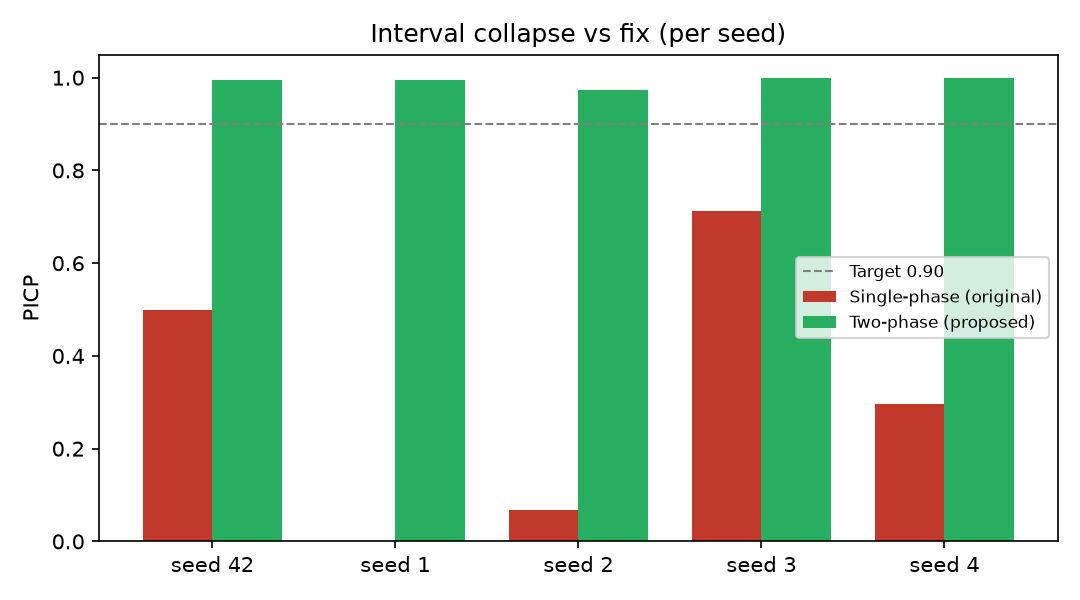
\includegraphics[width=\columnwidth]{figures/fig1_failfix.png}
  \caption{Per-seed interval coverage. Single-phase training (red) is unstable and frequently
  far below the $0.90$ target; two-phase training (green) is near-perfect across all seeds.}
  \label{fig:failfix}
\end{figure}

\begin{figure}[t]
  \centering
  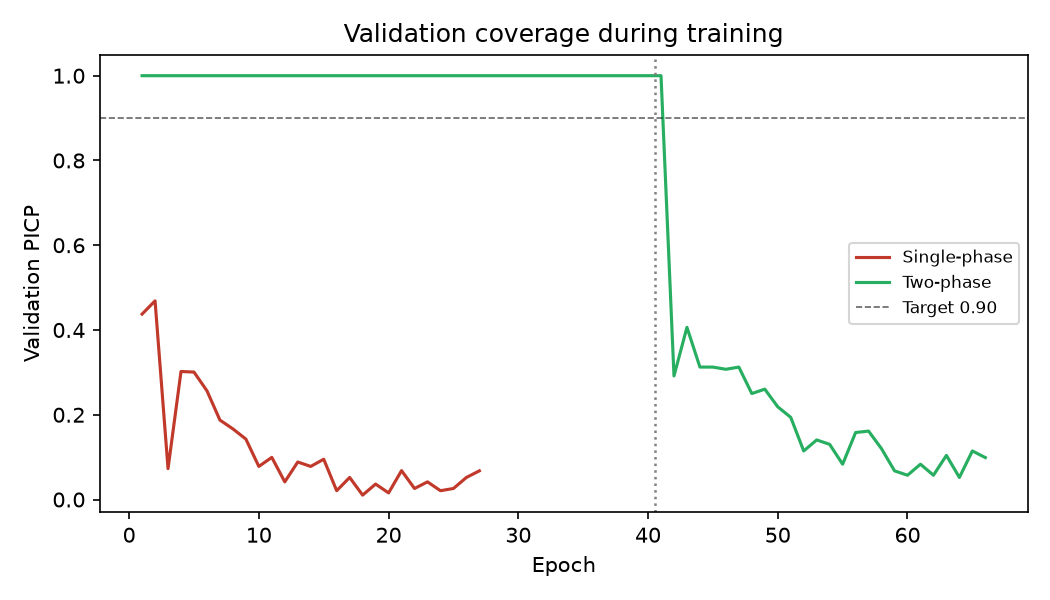
\includegraphics[width=\columnwidth]{figures/fig4_dynamics.png}
  \caption{Validation coverage during training. Single-phase coverage collapses early; the
  two-phase schedule keeps coverage high through the warm-up (dotted line) and recovers as
  interval learning proceeds.}
  \label{fig:dynamics}
\end{figure}

\begin{figure}[t]
  \centering
  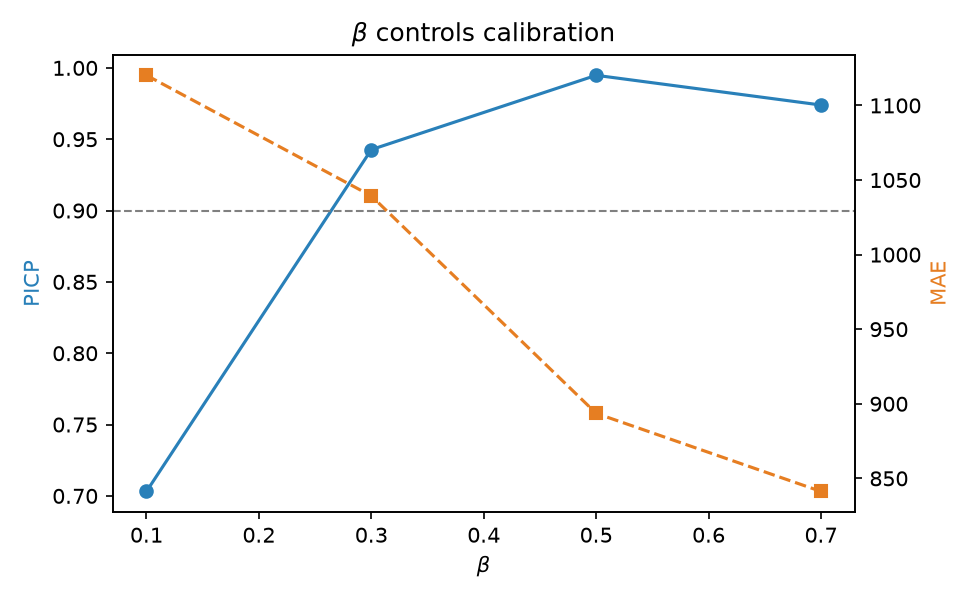
\includegraphics[width=\columnwidth]{figures/fig2_beta_sweep.png}
  \caption{Effect of the point-prediction weight $\beta$. Increasing $\beta$ raises PICP toward
  the target and lowers MAE, confirming $\beta$ (not $\lambda$) is the primary calibration lever.}
  \label{fig:beta}
\end{figure}

\begin{figure}[t]
  \centering
  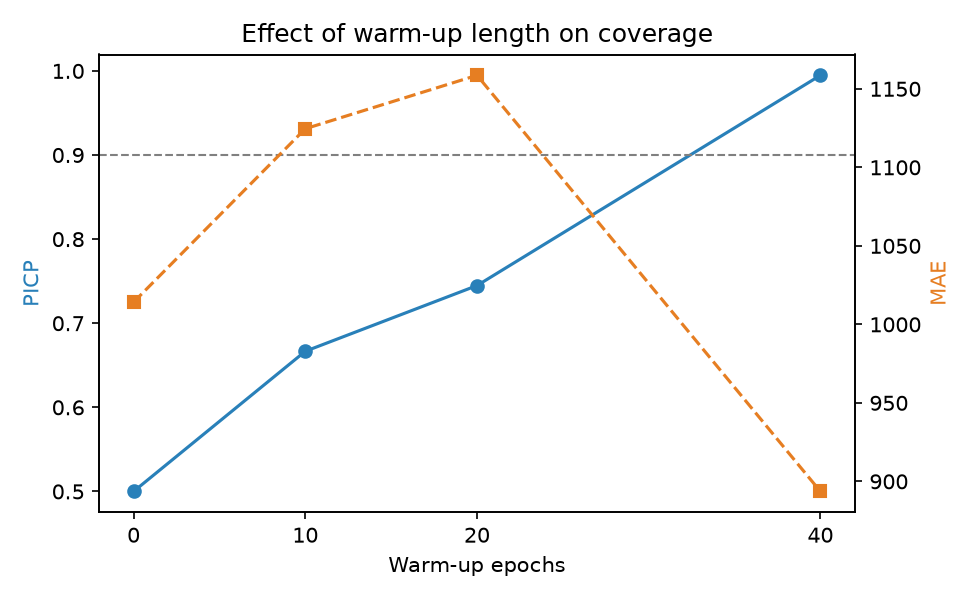
\includegraphics[width=\columnwidth]{figures/fig6_warmup.png}
  \caption{Warm-up length sweep. Longer point-only warm-up increases coverage; MAE is minimised
  at the longest warm-up, motivating the two-phase schedule.}
  \label{fig:warmup}
\end{figure}

\subsection{Residual gaps}
Two-phase training fixes collapse but not adaptiveness (Table~\ref{tab:gaps}). Split-conformal
calibration applies a single validation-residual quantile $\qhat$ globally; DeepPIPE-Ctrl
generalises this to $m_t\qhat$ with a learned $m_t$.

\begin{table}[t]
  \centering
  \caption{Residual calibration gaps motivating DeepPIPE-Ctrl.}
  \label{tab:gaps}
  \begin{tabular}{@{}clc@{}}
    \toprule
    Gap & Phenomenon & Evidence \\
    \midrule
    G1 & Volatility-blind widths & $\rho(\mathrm{width},\mathrm{VIX})=-0.50$ \\
    G2 & Regime-break under-coverage & Fold~1 PICP $=0.01$ \\
    G3 & Over-coverage, level-blind & PICP $\approx0.995$ \\
    \bottomrule
  \end{tabular}
\end{table}

%======================================================================
\section{DeepPIPE-Ctrl}
\label{sec:ctrl}
%======================================================================
\subsection{Controller architecture}
The two-phase DeepPIPE model and fold-local $\qhat$ are \emph{frozen}. At each test time $t$ the
controller observes state $\mathbf{s}_t\in\mathbb{R}^8$: VIX level and daily change (train
z-scores), realised volatility (5/20-day), momentum (5/20-day), OOD distance
$(\mathrm{Close}_t-\max_{\mathrm{train}}\mathrm{Close})/\max_{\mathrm{train}}$, and rolling mean
$|y-\hat{y}|$. All statistics are fold-local (no test leakage). Action $a_t$ selects
$m_t\in\mathcal{A}=\{0.5,0.75,1.0,1.25,1.5\}$ and
\begin{equation}
  L_t=\hat{y}_t-m_t\qhat,\qquad U_t=\hat{y}_t+m_t\qhat.
\end{equation}

\subsection{Contextual bandit formulation}
Because $m_t$ does not affect market dynamics, each step decouples into a contextual bandit with
context $\mathbf{s}_t$, action $m_t$, and reward $r_t=-S(L_t,U_t,y_{t+1})$, where $S$ is the
Winkler score at level $p$:
\begin{equation}
  S(L,U,y)=(U-L)+\tfrac{2}{\alpha}(L-y)\mathbb{1}[y<L]+\tfrac{2}{\alpha}(y-U)\mathbb{1}[y>U].
\end{equation}
Since $\hat{y}_t$, $\qhat$, and $y_{t+1}$ are known retrospectively, the full reward matrix
$\mathbf{R}\in\mathbb{R}^{N\times|\mathcal{A}|}$ is observable offline---no importance-weighted
off-policy estimation is required in v1.

\subsection{Policies and baselines}
\textbf{T0 (GreedyConstant):} single best constant multiplier.
\textbf{T1:} LinUCB / LinTS linear bandits on $\phi(\mathbf{s}_t)$.
\textbf{T2:} MLP softmax policy trained by reward regression.
\textbf{Static conformal:} $m_t\equiv1$.
\textbf{Conformal PID:} feedback on coverage error with clipped multipliers~\cite{angelopoulos2023pid}.

\subsection{Evaluation objectives}
\emph{Inner (statistical):} PICP, MPIW, mean normalised interval score, Kupiec POF, Christoffersen
independence, $\rho(\mathrm{width},\mathrm{VIX})$. \emph{Outer (economic):} a width-gated
long-only backtest where position size is inversely proportional to interval width; we report
Sharpe and max drawdown. P\&L is \emph{not} optimised during training; it is a downstream
consequence of calibration quality.

%======================================================================
\section{Experimental Setup}
\label{sec:experiments}
%======================================================================
\textbf{Data.} Daily NIFTY~50, 1{,}676 trading days (2020--2026), 14 core features (OHLCV, India
VIX, global indices, commodities, FX). Chronological split: 70\% train / 15\% val / 15\% test
($n_{\mathrm{test}}=192$).

\textbf{Training.} $L{=}60$, hidden 64, 2 layers, dropout 0.2, $\beta{=}0.5$, $\lambda{=}15$,
$p{=}0.90$, Adam lr $5{\times}10^{-4}$, Phase~1: 40 epochs, Phase~2: 120 epochs (early stop).

\textbf{Protocols.} E1--E10 cover the main comparison, fail/fix seeds, $\beta/\lambda$ sweeps,
feature ablation, robustness, rolling-window (5 folds), calibration tests, DM/bootstrap, VIX
analysis, conformal baseline, and training dynamics. E11--E14 cover controller inner metrics,
VIX--width, a rolling stress test, and the width-gated backtest. Experiments run in the
open-source \texttt{deeppipe} package (Python~3.10+, PyTorch~2.x) with YAML configuration and a
walk-forward harness.

%======================================================================
\section{Results}
\label{sec:results}
%======================================================================
\subsection{Two-phase baseline (E1--E2)}
Table~\ref{tab:e1} summarises the main test-set comparison. DeepPIPE two-phase achieves PICP
$0.995$ but MAE $893.6$, higher than naive baselines under OOD shift---consistent with
prioritising calibration over point accuracy. Table~\ref{tab:e2} shows the fail/fix contrast
across five seeds. Fig.~\ref{fig:intervals} visualises the resulting point forecast and 90\%
interval over the test period: the band expands during the sharp late-window drawdown, keeping
the realised close inside the interval.

\begin{figure}[t]
  \centering
  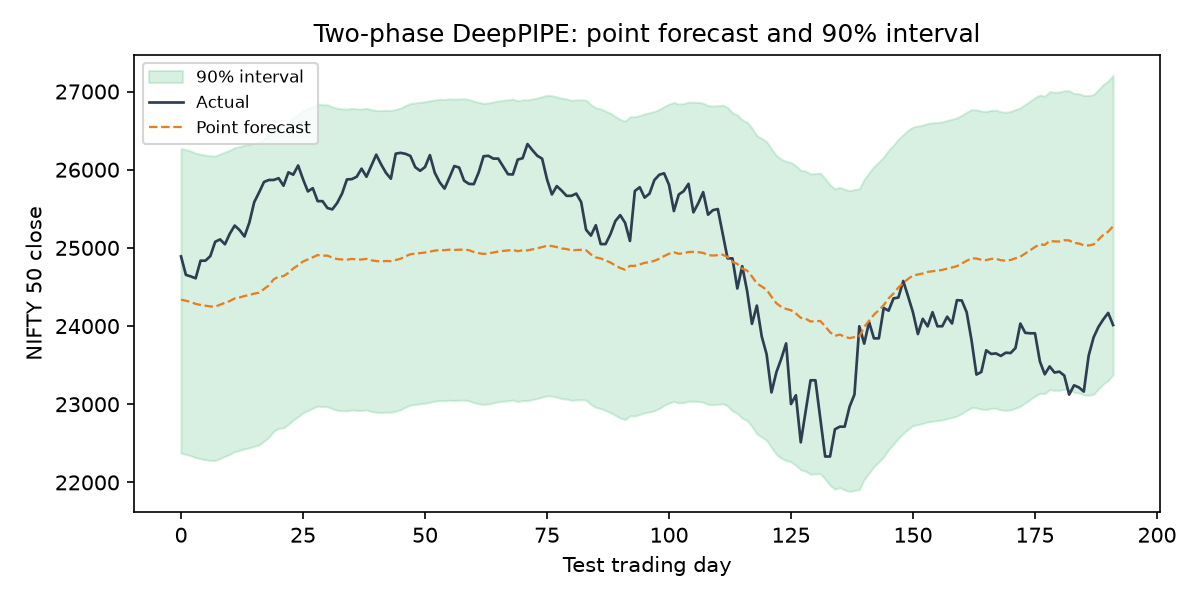
\includegraphics[width=\columnwidth]{figures/fig5_intervals.png}
  \caption{Two-phase DeepPIPE point forecast and 90\% prediction interval over the test period.
  The interval contains nearly all realised closes, including the volatile drawdown near day~130.}
  \label{fig:intervals}
\end{figure}

\begin{table}[t]
  \centering
  \caption{Main comparison on held-out test set (E1).}
  \label{tab:e1}
  \begin{tabular}{@{}lrrrr@{}}
    \toprule
    Model & MAE & RMSE & PICP & MPIW \\
    \midrule
    DeepPIPE (two-phase) & 893.6 & 984.8 & 0.995 & 3841.1 \\
    Naive                & 151.6 & 209.8 & ---   & --- \\
    Moving average (5)   & 235.5 & 302.9 & ---   & --- \\
    Linear regression    & 418.6 & 540.8 & ---   & --- \\
    GRU                  & 458.7 & 615.3 & ---   & --- \\
    LSTM                 & 2016.8 & 2155.7 & ---  & --- \\
    \bottomrule
  \end{tabular}
\end{table}

\begin{table}[t]
  \centering
  \caption{Single-phase vs.\ two-phase training (five seeds).}
  \label{tab:e2}
  \begin{tabular}{@{}lcc@{}}
    \toprule
    Metric & Single-phase & Two-phase \\
    \midrule
    PICP (mean $\pm$ std) & $0.32\pm0.27$ & $0.99\pm0.01$ \\
    MAE (mean)            & 1580.9        & 894.0 \\
    MPIW (mean)           & 1226.9        & 4121.8 \\
    \bottomrule
  \end{tabular}
\end{table}

\subsection{Volatility adaptiveness (E8)}
Two-phase DeepPIPE exhibits $\rho(\mathrm{width},\mathrm{VIX})=-0.50$; mean widths across
low/mid/high VIX terciles are nearly identical ($3861/3838/3824$), confirming gap~G1.

\subsection{DeepPIPE-Ctrl inner metrics (E11)}
Table~\ref{tab:e11} compares controllers on the static test split ($p{=}0.90$). Conformal PID is
closest to target coverage and reverses the VIX--width sign. T0 matches static conformal exactly,
so no constant $m\neq1$ helps here. Learned bandits underperform PID on interval score; T2 severely
under-covers.

\begin{table}[t]
  \centering
  \caption{Adaptive calibration methods ($n{=}192$, target PICP $0.90$).}
  \label{tab:e11}
  \begin{tabular}{@{}lrrrr@{}}
    \toprule
    Method & PICP & MPIW & Score & $\rho_{w,\mathrm{VIX}}$ \\
    \midrule
    Static conformal / T0 & 0.885 & 2694.5 & 2.39 & --- \\
    Conformal PID         & \textbf{0.901} & 3193.9 & 2.54 & \textbf{0.020} \\
    LinUCB (T1)           & 0.865 & 2820.3 & 2.68 & $-0.42$ \\
    LinTS (T1)            & 0.844 & 2810.9 & 2.67 & $-0.36$ \\
    MLP (T2)              & 0.719 & 2552.9 & 3.30 & $-0.58$ \\
    \bottomrule
  \end{tabular}
\end{table}

\subsection{Rolling-window stress test (E13)}
On Fold~1 (prices $21.8\mathrm{k}\rightarrow26.0\mathrm{k}$), LinUCB PICP improves from $0.011$
(static) to $0.033$---directionally better but far from $0.90$. On stable folds, LinUCB matches or
marginally improves normalised interval score. Fig.~\ref{fig:rolling} makes the mechanism
explicit: coverage collapses precisely on the fold whose maximum price exceeds the training
maximum (24{,}613), confirming gap~G2.

\begin{figure}[t]
  \centering
  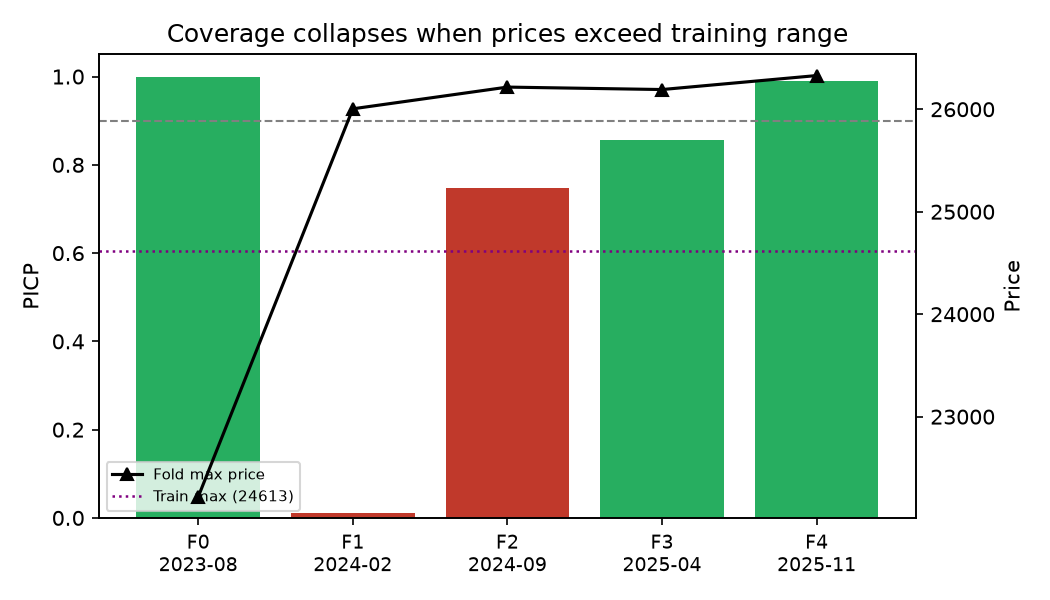
\includegraphics[width=\columnwidth]{figures/fig3_rolling.png}
  \caption{Walk-forward coverage per fold (bars) against each fold's maximum price (line).
  Coverage collapses on the fold that first breaches the training price ceiling.}
  \label{fig:rolling}
\end{figure}

\subsection{Width-gated backtest (E14)}
Table~\ref{tab:e14} reports the outer economic metrics. All Sharpe ratios are negative on this OOD
window; PID is least negative, aligning with its superior inner calibration.

\begin{table}[t]
  \centering
  \caption{Outer economic metrics, width-gated strategy.}
  \label{tab:e14}
  \begin{tabular}{@{}lrrr@{}}
    \toprule
    Method & Ann.\ return & Sharpe & Max DD \\
    \midrule
    Static conformal / T0 & $-3.8\%$ & $-0.27$ & $-15.2\%$ \\
    Conformal PID         & $-1.6\%$ & $-0.12$ & $-14.1\%$ \\
    LinUCB                & $-7.3\%$ & $-0.58$ & $-14.6\%$ \\
    MLP                   & $-4.8\%$ & $-0.36$ & $-14.8\%$ \\
    \bottomrule
  \end{tabular}
\end{table}

%======================================================================
\section{Discussion}
\label{sec:discussion}
%======================================================================
\textbf{Training vs.\ calibration.} Results support a two-layer view: two-phase training repairs
\emph{optimisation-induced} interval collapse, while adaptive conformal methods address
\emph{post-hoc} miscalibration. They are complementary; static split-conformal after two-phase
training still over-covers and ignores volatility state.

\textbf{Learned vs.\ hand-crafted control.} With only $\sim$190 validation and $\sim$192 test
points per fold, linear bandits and MLPs lack data to beat a well-tuned PID controller. This is an
honest negative result: adaptive width need not require learning if a simple feedback law
suffices. Future work should add coverage-error memory (a true MDP), asymmetric bounds, and online
updates (ACI/CQL).

\textbf{Limitations.} The controller rescales width around a possibly biased $\hat{y}$; it does not
correct location error. The economic evaluation is illustrative, not a trading objective. Results
cover one index and one shift pattern; broader asset panels would strengthen external validity.

%======================================================================
\section{Conclusion}
\label{sec:conclusion}
%======================================================================
We showed that single-phase DeepPIPE training fails under a documented NIFTY~50 distribution shift
while two-phase training restores coverage. We then introduced DeepPIPE-Ctrl, formulating adaptive
conformal width control as a Winkler-driven contextual bandit with exogenous market state.
Conformal PID currently dominates learned policies on calibration metrics; bandit policies show
modest gains only under extreme rolling regimes. Together, two-phase training plus adaptive
calibration form a practical pipeline for uncertainty-aware forecasting under shift, with
open-source code for full reproduction.

\section*{Acknowledgements}
The authors thank Prof.\ Jabez Christopher and Prof.\ Vasan Arunachalam for their guidance.

\section*{Author Contributions}
Problem framing, the contextual-bandit formulation, Winkler reward design, state-feature
selection, the walk-forward protocol, and the experiment matrix were developed jointly by all
three authors. All subsequent implementation, experimentation, analysis, and writing were divided
equally ($\sim$33\% each), with mutual cross-review before integration.

\begin{thebibliography}{9}
\bibitem{wang2020deeppipe}
H.~Wang, X.~Xu, Z.~Wang, and K.~K.~Lai, ``Deep prediction intervals,''
\emph{Neurocomputing}, vol.~397, pp.~10--23, 2020.

\bibitem{gneiting2007scoring}
T.~Gneiting and A.~E.~Raftery, ``Strictly proper scoring rules, prediction, and estimation,''
\emph{J.\ Amer.\ Stat.\ Assoc.}, vol.~102, no.~477, pp.~359--378, 2007.

\bibitem{romano2019cqr}
Y.~Romano, E.~Patterson, and E.~J.~Cand\`es, ``Conformalized quantile regression,''
in \emph{Adv.\ Neural Inf.\ Process.\ Syst.}, vol.~32, 2019.

\bibitem{gibbs2021aci}
I.~Gibbs and E.~J.~Cand\`es, ``Adaptive conformal inference under distribution shift,''
in \emph{Adv.\ Neural Inf.\ Process.\ Syst.}, vol.~34, 2021.

\bibitem{angelopoulos2023pid}
A.~N.~Angelopoulos, E.~J.~Cand\`es, and R.~J.~Tibshirani, ``Conformal PID control for time series
prediction,'' \emph{arXiv:2307.16895}, 2023.

\bibitem{zhou2021informer}
H.~Zhou \emph{et al.}, ``Informer: Beyond efficient transformer for long sequence time-series
forecasting,'' in \emph{Proc.\ AAAI}, vol.~35, no.~12, pp.~11106--11115, 2021.

\bibitem{lim2021tft}
B.~Lim, S.~O.~Ar{\i}k, N.~Loeff, and T.~Pfister, ``Temporal fusion transformers for interpretable
multi-horizon time series forecasting,'' \emph{Int.\ J.\ Forecast.}, vol.~37, no.~4,
pp.~1748--1764, 2021.

\bibitem{zeng2023dlinear}
A.~Zeng, M.~Chen, L.~Zhang, and Q.~Xu, ``Are transformers effective for time series
forecasting?'' in \emph{Proc.\ AAAI}, vol.~37, no.~9, pp.~11121--11128, 2023.
\end{thebibliography}

\end{document}
